% This file is generated by the MATLAB m-file laprint.m. It can be included
% into LaTeX documents using the packages graphicx, color and psfrag.
% It is accompanied by a postscript file. A sample LaTeX file is:
%    \documentclass{article}\usepackage{graphicx,color,psfrag}
%    \begin{document}% This file is generated by the MATLAB m-file laprint.m. It can be included
% into LaTeX documents using the packages graphicx, color and psfrag.
% It is accompanied by a postscript file. A sample LaTeX file is:
%    \documentclass{article}\usepackage{graphicx,color,psfrag}
%    \begin{document}% This file is generated by the MATLAB m-file laprint.m. It can be included
% into LaTeX documents using the packages graphicx, color and psfrag.
% It is accompanied by a postscript file. A sample LaTeX file is:
%    \documentclass{article}\usepackage{graphicx,color,psfrag}
%    \begin{document}% This file is generated by the MATLAB m-file laprint.m. It can be included
% into LaTeX documents using the packages graphicx, color and psfrag.
% It is accompanied by a postscript file. A sample LaTeX file is:
%    \documentclass{article}\usepackage{graphicx,color,psfrag}
%    \begin{document}\input{Example76l}\end{document}
% See http://www.mathworks.de/matlabcentral/fileexchange/loadFile.do?objectId=4638
% for recent versions of laprint.m.
%
% created by:           LaPrint version 3.16 (13.9.2004)
% created on:           25-Oct-2009 09:23:03
% eps bounding box:     7.5 cm x 4.5712 cm
% comment:              
%
\begin{psfrags}%
\psfragscanon%
%
% text strings:
\psfrag{s05}[t][t]{\color[rgb]{0,0,0}\setlength{\tabcolsep}{0pt}\begin{tabular}{c}$x_1$\end{tabular}}%
\psfrag{s06}[b][b]{\color[rgb]{0,0,0}\setlength{\tabcolsep}{0pt}\begin{tabular}{c}$x_2$\end{tabular}}%
\psfrag{s07}[l][l]{\color[rgb]{0,0,0}\setlength{\tabcolsep}{0pt}\begin{tabular}{l}CR1\end{tabular}}%
\psfrag{s08}[l][l]{\color[rgb]{0,0,0}\setlength{\tabcolsep}{0pt}\begin{tabular}{l}CR2\end{tabular}}%
\psfrag{s09}[l][l]{\color[rgb]{0,0,0}\setlength{\tabcolsep}{0pt}\begin{tabular}{l}CR3\end{tabular}}%
\psfrag{s10}[l][l]{\color[rgb]{0,0,0}\setlength{\tabcolsep}{0pt}\begin{tabular}{l}CR4\end{tabular}}%
\psfrag{s11}[l][l]{\color[rgb]{0,0,0}\setlength{\tabcolsep}{0pt}\begin{tabular}{l}CR5\end{tabular}}%
\psfrag{s12}[l][l]{\color[rgb]{0,0,0}\setlength{\tabcolsep}{0pt}\begin{tabular}{l}CR6\end{tabular}}%
\psfrag{s13}[l][l]{\color[rgb]{0,0,0}\setlength{\tabcolsep}{0pt}\begin{tabular}{l}CR7\end{tabular}}%
\psfrag{s14}[l][l]{\color[rgb]{0,0,0}\setlength{\tabcolsep}{0pt}\begin{tabular}{l}CR8\end{tabular}}%
\psfrag{s15}[l][l]{\color[rgb]{0,0,0}\setlength{\tabcolsep}{0pt}\begin{tabular}{l}CR9\end{tabular}}%
\psfrag{s16}[l][l]{\color[rgb]{0,0,0}\setlength{\tabcolsep}{0pt}\begin{tabular}{l}CR10\end{tabular}}%
\psfrag{s17}[l][l]{\color[rgb]{0,0,0}\setlength{\tabcolsep}{0pt}\begin{tabular}{l}CR11\end{tabular}}%
\psfrag{s18}[l][l]{\color[rgb]{0,0,0}\setlength{\tabcolsep}{0pt}\begin{tabular}{l}CR12\end{tabular}}%
\psfrag{s19}[l][l]{\color[rgb]{0,0,0}\setlength{\tabcolsep}{0pt}\begin{tabular}{l}CR13\end{tabular}}%
\psfrag{s20}[l][l]{\color[rgb]{0,0,0}\setlength{\tabcolsep}{0pt}\begin{tabular}{l}CR14\end{tabular}}%
\psfrag{s21}[l][l]{\color[rgb]{0,0,0}\setlength{\tabcolsep}{0pt}\begin{tabular}{l}CR15\end{tabular}}%
\psfrag{s22}[l][l]{\color[rgb]{0,0,0}\setlength{\tabcolsep}{0pt}\begin{tabular}{l}CR16\end{tabular}}%
\psfrag{s23}[l][l]{\color[rgb]{0,0,0}\setlength{\tabcolsep}{0pt}\begin{tabular}{l}CR17\end{tabular}}%
%
% xticklabels:
\psfrag{x01}[t][t]{0}%
\psfrag{x02}[t][t]{0.2}%
\psfrag{x03}[t][t]{0.4}%
\psfrag{x04}[t][t]{0.6}%
\psfrag{x05}[t][t]{0.8}%
\psfrag{x06}[t][t]{1}%
\psfrag{x07}[t][t]{-10}%
\psfrag{x08}[t][t]{-5}%
\psfrag{x09}[t][t]{0}%
\psfrag{x10}[t][t]{5}%
\psfrag{x11}[t][t]{10}%
%
% yticklabels:
\psfrag{v01}[r][r]{0}%
\psfrag{v02}[r][r]{0.2}%
\psfrag{v03}[r][r]{0.4}%
\psfrag{v04}[r][r]{0.6}%
\psfrag{v05}[r][r]{0.8}%
\psfrag{v06}[r][r]{1}%
\psfrag{v07}[r][r]{-10}%
\psfrag{v08}[r][r]{-5}%
\psfrag{v09}[r][r]{0}%
\psfrag{v10}[r][r]{5}%
\psfrag{v11}[r][r]{10}%
%
% Figure:
\resizebox{6cm}{!}{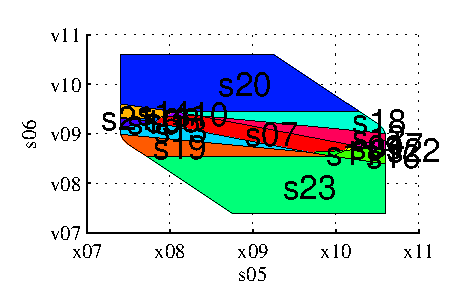
\includegraphics{Example76l.eps}}%
\end{psfrags}%
%
% End Example76l.tex
\end{document}
% See http://www.mathworks.de/matlabcentral/fileexchange/loadFile.do?objectId=4638
% for recent versions of laprint.m.
%
% created by:           LaPrint version 3.16 (13.9.2004)
% created on:           25-Oct-2009 09:23:03
% eps bounding box:     7.5 cm x 4.5712 cm
% comment:              
%
\begin{psfrags}%
\psfragscanon%
%
% text strings:
\psfrag{s05}[t][t]{\color[rgb]{0,0,0}\setlength{\tabcolsep}{0pt}\begin{tabular}{c}$x_1$\end{tabular}}%
\psfrag{s06}[b][b]{\color[rgb]{0,0,0}\setlength{\tabcolsep}{0pt}\begin{tabular}{c}$x_2$\end{tabular}}%
\psfrag{s07}[l][l]{\color[rgb]{0,0,0}\setlength{\tabcolsep}{0pt}\begin{tabular}{l}CR1\end{tabular}}%
\psfrag{s08}[l][l]{\color[rgb]{0,0,0}\setlength{\tabcolsep}{0pt}\begin{tabular}{l}CR2\end{tabular}}%
\psfrag{s09}[l][l]{\color[rgb]{0,0,0}\setlength{\tabcolsep}{0pt}\begin{tabular}{l}CR3\end{tabular}}%
\psfrag{s10}[l][l]{\color[rgb]{0,0,0}\setlength{\tabcolsep}{0pt}\begin{tabular}{l}CR4\end{tabular}}%
\psfrag{s11}[l][l]{\color[rgb]{0,0,0}\setlength{\tabcolsep}{0pt}\begin{tabular}{l}CR5\end{tabular}}%
\psfrag{s12}[l][l]{\color[rgb]{0,0,0}\setlength{\tabcolsep}{0pt}\begin{tabular}{l}CR6\end{tabular}}%
\psfrag{s13}[l][l]{\color[rgb]{0,0,0}\setlength{\tabcolsep}{0pt}\begin{tabular}{l}CR7\end{tabular}}%
\psfrag{s14}[l][l]{\color[rgb]{0,0,0}\setlength{\tabcolsep}{0pt}\begin{tabular}{l}CR8\end{tabular}}%
\psfrag{s15}[l][l]{\color[rgb]{0,0,0}\setlength{\tabcolsep}{0pt}\begin{tabular}{l}CR9\end{tabular}}%
\psfrag{s16}[l][l]{\color[rgb]{0,0,0}\setlength{\tabcolsep}{0pt}\begin{tabular}{l}CR10\end{tabular}}%
\psfrag{s17}[l][l]{\color[rgb]{0,0,0}\setlength{\tabcolsep}{0pt}\begin{tabular}{l}CR11\end{tabular}}%
\psfrag{s18}[l][l]{\color[rgb]{0,0,0}\setlength{\tabcolsep}{0pt}\begin{tabular}{l}CR12\end{tabular}}%
\psfrag{s19}[l][l]{\color[rgb]{0,0,0}\setlength{\tabcolsep}{0pt}\begin{tabular}{l}CR13\end{tabular}}%
\psfrag{s20}[l][l]{\color[rgb]{0,0,0}\setlength{\tabcolsep}{0pt}\begin{tabular}{l}CR14\end{tabular}}%
\psfrag{s21}[l][l]{\color[rgb]{0,0,0}\setlength{\tabcolsep}{0pt}\begin{tabular}{l}CR15\end{tabular}}%
\psfrag{s22}[l][l]{\color[rgb]{0,0,0}\setlength{\tabcolsep}{0pt}\begin{tabular}{l}CR16\end{tabular}}%
\psfrag{s23}[l][l]{\color[rgb]{0,0,0}\setlength{\tabcolsep}{0pt}\begin{tabular}{l}CR17\end{tabular}}%
%
% xticklabels:
\psfrag{x01}[t][t]{0}%
\psfrag{x02}[t][t]{0.2}%
\psfrag{x03}[t][t]{0.4}%
\psfrag{x04}[t][t]{0.6}%
\psfrag{x05}[t][t]{0.8}%
\psfrag{x06}[t][t]{1}%
\psfrag{x07}[t][t]{-10}%
\psfrag{x08}[t][t]{-5}%
\psfrag{x09}[t][t]{0}%
\psfrag{x10}[t][t]{5}%
\psfrag{x11}[t][t]{10}%
%
% yticklabels:
\psfrag{v01}[r][r]{0}%
\psfrag{v02}[r][r]{0.2}%
\psfrag{v03}[r][r]{0.4}%
\psfrag{v04}[r][r]{0.6}%
\psfrag{v05}[r][r]{0.8}%
\psfrag{v06}[r][r]{1}%
\psfrag{v07}[r][r]{-10}%
\psfrag{v08}[r][r]{-5}%
\psfrag{v09}[r][r]{0}%
\psfrag{v10}[r][r]{5}%
\psfrag{v11}[r][r]{10}%
%
% Figure:
\resizebox{6cm}{!}{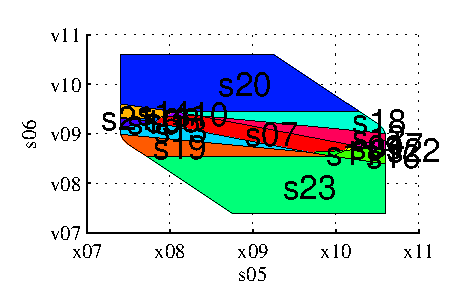
\includegraphics{Example76l.eps}}%
\end{psfrags}%
%
% End Example76l.tex
\end{document}
% See http://www.mathworks.de/matlabcentral/fileexchange/loadFile.do?objectId=4638
% for recent versions of laprint.m.
%
% created by:           LaPrint version 3.16 (13.9.2004)
% created on:           25-Oct-2009 09:23:03
% eps bounding box:     7.5 cm x 4.5712 cm
% comment:              
%
\begin{psfrags}%
\psfragscanon%
%
% text strings:
\psfrag{s05}[t][t]{\color[rgb]{0,0,0}\setlength{\tabcolsep}{0pt}\begin{tabular}{c}$x_1$\end{tabular}}%
\psfrag{s06}[b][b]{\color[rgb]{0,0,0}\setlength{\tabcolsep}{0pt}\begin{tabular}{c}$x_2$\end{tabular}}%
\psfrag{s07}[l][l]{\color[rgb]{0,0,0}\setlength{\tabcolsep}{0pt}\begin{tabular}{l}CR1\end{tabular}}%
\psfrag{s08}[l][l]{\color[rgb]{0,0,0}\setlength{\tabcolsep}{0pt}\begin{tabular}{l}CR2\end{tabular}}%
\psfrag{s09}[l][l]{\color[rgb]{0,0,0}\setlength{\tabcolsep}{0pt}\begin{tabular}{l}CR3\end{tabular}}%
\psfrag{s10}[l][l]{\color[rgb]{0,0,0}\setlength{\tabcolsep}{0pt}\begin{tabular}{l}CR4\end{tabular}}%
\psfrag{s11}[l][l]{\color[rgb]{0,0,0}\setlength{\tabcolsep}{0pt}\begin{tabular}{l}CR5\end{tabular}}%
\psfrag{s12}[l][l]{\color[rgb]{0,0,0}\setlength{\tabcolsep}{0pt}\begin{tabular}{l}CR6\end{tabular}}%
\psfrag{s13}[l][l]{\color[rgb]{0,0,0}\setlength{\tabcolsep}{0pt}\begin{tabular}{l}CR7\end{tabular}}%
\psfrag{s14}[l][l]{\color[rgb]{0,0,0}\setlength{\tabcolsep}{0pt}\begin{tabular}{l}CR8\end{tabular}}%
\psfrag{s15}[l][l]{\color[rgb]{0,0,0}\setlength{\tabcolsep}{0pt}\begin{tabular}{l}CR9\end{tabular}}%
\psfrag{s16}[l][l]{\color[rgb]{0,0,0}\setlength{\tabcolsep}{0pt}\begin{tabular}{l}CR10\end{tabular}}%
\psfrag{s17}[l][l]{\color[rgb]{0,0,0}\setlength{\tabcolsep}{0pt}\begin{tabular}{l}CR11\end{tabular}}%
\psfrag{s18}[l][l]{\color[rgb]{0,0,0}\setlength{\tabcolsep}{0pt}\begin{tabular}{l}CR12\end{tabular}}%
\psfrag{s19}[l][l]{\color[rgb]{0,0,0}\setlength{\tabcolsep}{0pt}\begin{tabular}{l}CR13\end{tabular}}%
\psfrag{s20}[l][l]{\color[rgb]{0,0,0}\setlength{\tabcolsep}{0pt}\begin{tabular}{l}CR14\end{tabular}}%
\psfrag{s21}[l][l]{\color[rgb]{0,0,0}\setlength{\tabcolsep}{0pt}\begin{tabular}{l}CR15\end{tabular}}%
\psfrag{s22}[l][l]{\color[rgb]{0,0,0}\setlength{\tabcolsep}{0pt}\begin{tabular}{l}CR16\end{tabular}}%
\psfrag{s23}[l][l]{\color[rgb]{0,0,0}\setlength{\tabcolsep}{0pt}\begin{tabular}{l}CR17\end{tabular}}%
%
% xticklabels:
\psfrag{x01}[t][t]{0}%
\psfrag{x02}[t][t]{0.2}%
\psfrag{x03}[t][t]{0.4}%
\psfrag{x04}[t][t]{0.6}%
\psfrag{x05}[t][t]{0.8}%
\psfrag{x06}[t][t]{1}%
\psfrag{x07}[t][t]{-10}%
\psfrag{x08}[t][t]{-5}%
\psfrag{x09}[t][t]{0}%
\psfrag{x10}[t][t]{5}%
\psfrag{x11}[t][t]{10}%
%
% yticklabels:
\psfrag{v01}[r][r]{0}%
\psfrag{v02}[r][r]{0.2}%
\psfrag{v03}[r][r]{0.4}%
\psfrag{v04}[r][r]{0.6}%
\psfrag{v05}[r][r]{0.8}%
\psfrag{v06}[r][r]{1}%
\psfrag{v07}[r][r]{-10}%
\psfrag{v08}[r][r]{-5}%
\psfrag{v09}[r][r]{0}%
\psfrag{v10}[r][r]{5}%
\psfrag{v11}[r][r]{10}%
%
% Figure:
\resizebox{6cm}{!}{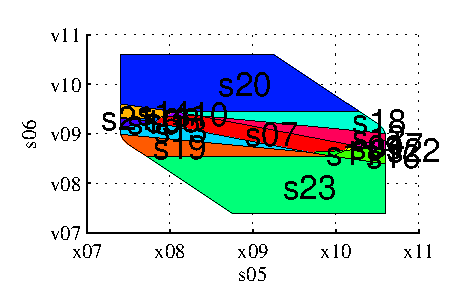
\includegraphics{Example76l.eps}}%
\end{psfrags}%
%
% End Example76l.tex
\end{document}
% See http://www.mathworks.de/matlabcentral/fileexchange/loadFile.do?objectId=4638
% for recent versions of laprint.m.
%
% created by:           LaPrint version 3.16 (13.9.2004)
% created on:           25-Oct-2009 09:23:03
% eps bounding box:     7.5 cm x 4.5712 cm
% comment:              
%
\begin{psfrags}%
\psfragscanon%
%
% text strings:
\psfrag{s05}[t][t]{\color[rgb]{0,0,0}\setlength{\tabcolsep}{0pt}\begin{tabular}{c}$x_1$\end{tabular}}%
\psfrag{s06}[b][b]{\color[rgb]{0,0,0}\setlength{\tabcolsep}{0pt}\begin{tabular}{c}$x_2$\end{tabular}}%
\psfrag{s07}[l][l]{\color[rgb]{0,0,0}\setlength{\tabcolsep}{0pt}\begin{tabular}{l}CR1\end{tabular}}%
\psfrag{s08}[l][l]{\color[rgb]{0,0,0}\setlength{\tabcolsep}{0pt}\begin{tabular}{l}CR2\end{tabular}}%
\psfrag{s09}[l][l]{\color[rgb]{0,0,0}\setlength{\tabcolsep}{0pt}\begin{tabular}{l}CR3\end{tabular}}%
\psfrag{s10}[l][l]{\color[rgb]{0,0,0}\setlength{\tabcolsep}{0pt}\begin{tabular}{l}CR4\end{tabular}}%
\psfrag{s11}[l][l]{\color[rgb]{0,0,0}\setlength{\tabcolsep}{0pt}\begin{tabular}{l}CR5\end{tabular}}%
\psfrag{s12}[l][l]{\color[rgb]{0,0,0}\setlength{\tabcolsep}{0pt}\begin{tabular}{l}CR6\end{tabular}}%
\psfrag{s13}[l][l]{\color[rgb]{0,0,0}\setlength{\tabcolsep}{0pt}\begin{tabular}{l}CR7\end{tabular}}%
\psfrag{s14}[l][l]{\color[rgb]{0,0,0}\setlength{\tabcolsep}{0pt}\begin{tabular}{l}CR8\end{tabular}}%
\psfrag{s15}[l][l]{\color[rgb]{0,0,0}\setlength{\tabcolsep}{0pt}\begin{tabular}{l}CR9\end{tabular}}%
\psfrag{s16}[l][l]{\color[rgb]{0,0,0}\setlength{\tabcolsep}{0pt}\begin{tabular}{l}CR10\end{tabular}}%
\psfrag{s17}[l][l]{\color[rgb]{0,0,0}\setlength{\tabcolsep}{0pt}\begin{tabular}{l}CR11\end{tabular}}%
\psfrag{s18}[l][l]{\color[rgb]{0,0,0}\setlength{\tabcolsep}{0pt}\begin{tabular}{l}CR12\end{tabular}}%
\psfrag{s19}[l][l]{\color[rgb]{0,0,0}\setlength{\tabcolsep}{0pt}\begin{tabular}{l}CR13\end{tabular}}%
\psfrag{s20}[l][l]{\color[rgb]{0,0,0}\setlength{\tabcolsep}{0pt}\begin{tabular}{l}CR14\end{tabular}}%
\psfrag{s21}[l][l]{\color[rgb]{0,0,0}\setlength{\tabcolsep}{0pt}\begin{tabular}{l}CR15\end{tabular}}%
\psfrag{s22}[l][l]{\color[rgb]{0,0,0}\setlength{\tabcolsep}{0pt}\begin{tabular}{l}CR16\end{tabular}}%
\psfrag{s23}[l][l]{\color[rgb]{0,0,0}\setlength{\tabcolsep}{0pt}\begin{tabular}{l}CR17\end{tabular}}%
%
% xticklabels:
\psfrag{x01}[t][t]{0}%
\psfrag{x02}[t][t]{0.2}%
\psfrag{x03}[t][t]{0.4}%
\psfrag{x04}[t][t]{0.6}%
\psfrag{x05}[t][t]{0.8}%
\psfrag{x06}[t][t]{1}%
\psfrag{x07}[t][t]{-10}%
\psfrag{x08}[t][t]{-5}%
\psfrag{x09}[t][t]{0}%
\psfrag{x10}[t][t]{5}%
\psfrag{x11}[t][t]{10}%
%
% yticklabels:
\psfrag{v01}[r][r]{0}%
\psfrag{v02}[r][r]{0.2}%
\psfrag{v03}[r][r]{0.4}%
\psfrag{v04}[r][r]{0.6}%
\psfrag{v05}[r][r]{0.8}%
\psfrag{v06}[r][r]{1}%
\psfrag{v07}[r][r]{-10}%
\psfrag{v08}[r][r]{-5}%
\psfrag{v09}[r][r]{0}%
\psfrag{v10}[r][r]{5}%
\psfrag{v11}[r][r]{10}%
%
% Figure:
\resizebox{6cm}{!}{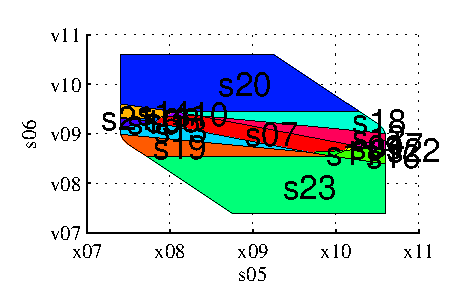
\includegraphics{Example76l.eps}}%
\end{psfrags}%
%
% End Example76l.tex
